%        File: 19.03.20.tex
%     Created: чт мар 19 08:00  2020 M
% Last Change: чт мар 19 08:00  2020 M
%
\documentclass[algebra,twocolumn]{pum}
\listnumber{1}
\date{19.03.20}
\classname{8-Д}
\lesson{10:30-12:20 }
\begin{document}
\subsubsection*{Прямая пропорциональность}

  Функция $y=kx$ называется прямой пропорциональностью. Ее графиком является прямая линия, проходящая через начало координат. Постоянный множитель $k$ называется коэффициентом пропорциональности. Если $k=1$ функция называется \emph{тождественной}.

  \begin{center} 
    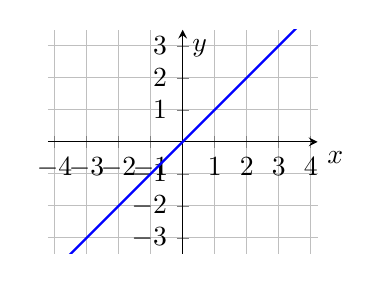
\begin{tikzpicture}
      \begin{axis}[
          scale=0.5,
          xmin=-1.5, xmax=1.5,
          ymin=-3.5, ymax=3.5,
          axis lines=middle,
          axis equal,
          grid=both,
          xtick distance=1,
          ytick distance=1,
          xlabel=$x$,
          ylabel=$y$,
          xlabel style={at={(ticklabel* cs:1)}, anchor=north west},
          ylabel style={at={(ticklabel* cs:1)}, anchor=north west}
        ]
        \addplot[blue,mark=none,thick=8pt] {x};
%  \addplot[blue,mark=none,thick=8pt, domain=-5:-0.2] {1/x};
%  \addplot[blue,mark=none,thick=8pt, domain=0.2:5] {1/x};
      \end{axis}
    \end{tikzpicture}
  \end{center}

  Свойства графика тождественной функции:
  \begin{enumerate}[nosep]
    \item График функции лежит в I и III координатных четвертях.
    \item График функции чертится движением карандаша/ручки слева направо снизу вверх.
    \item У графика функции нет \emph{асимптот}.
    \item Движение карандаша/ручки происходит без отрыва от бумаги. 
  \end{enumerate}

  Асимптота -- прямая, которая никогда не пересекается с графиком функции, но проходит от него на любом сколь угодно малом расстоянии.

  \begin{exercises}
    \begin{question}
      Построить график функции
      \begin{multicols}{3}
        \begin{enumerate}[label=\arabic*)]
        \item $y=2x$ 
        \item $y=4x$ 
        \item $y=\frac{1}{2}x$ 
        \item $y=\frac{1}{2}x$ 
        \item $y=-2x$ 
        \item $y=-\frac{1}{2}x$ 
      \end{enumerate}
    \end{multicols}
  \end{question}
  \begin{question}
    Принадлежат ли графику каждой из построенных функций точки:\\
    A(2; 1), B(12; -4), C(0,3; -16), D (0,4; -120).
  \end{question}
  \begin{question}
    По графику найти абсциссу точки графика построенных функций с ординатой: 10; -6; $\frac{10}{6}$.
  \end{question}
  \begin{question}
    По графику найти ординату точки графика построенных функций с абсциссой: -3; $\frac{1}{4}$; 0,2.
  \end{question}
\end{exercises}

\subsubsection*{Замечания по выполненным построениям}

\begin{center}
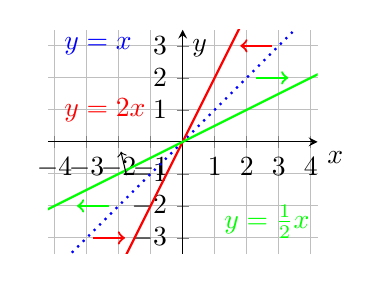
\begin{tikzpicture}
\begin{axis}[
    scale=0.5,
    xmin=-1.5, xmax=1.5,
    ymin=-3.5, ymax=3.5,
    axis lines=middle,
    axis equal,
    grid=both,
    xtick distance=1,
    ytick distance=1,
    xlabel=$x$,
    ylabel=$y$,
    xlabel style={at={(ticklabel* cs:1)}, anchor=north west},
    ylabel style={at={(ticklabel* cs:1)}, anchor=north west}
  ]
  \addplot[blue,mark=none,dotted,thick=8pt] {x};
  \addplot[red,mark=none,thick=8pt] {2*x};
  \addplot[green,mark=none,thick=8pt] {0.5*x};
  \node[blue,right] at (axis cs: -4,3) {$y=x$};
  \node[red,right] at (axis cs: -4,1) {$y=2x$};
  \node[green,right] at (axis cs: 1,-2.5) {$y=\frac{1}{2}x$};
  \draw[->,red,thick] (axis cs: 2.8,3) -- (axis cs: 1.8,3);
  \draw[->,red,thick] (axis cs: -2.8,-3) -- (axis cs: -1.8,-3);
  \draw[<-,green,thick] (axis cs: 3.3,2) -- (axis cs: 2.3,2);
  \draw[<-,green,thick] (axis cs: -3.3,-2) -- (axis cs: -2.3,-2);
  \node (horizont) at (axis cs: -2,0) {};
  \node (vertical) at (axis cs: 0,-2) {};
\end{axis}
\draw[->] (1,1) -- (horizont);
\end{tikzpicture}
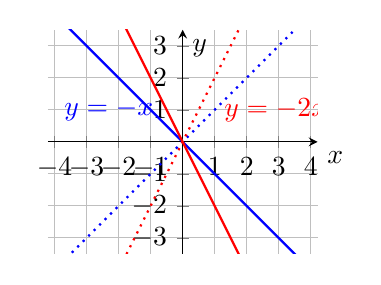
\begin{tikzpicture}
\begin{axis}[
    scale=0.5,
    xmin=-1.5, xmax=1.5,
    ymin=-3.5, ymax=3.5,
    axis lines=middle,
    axis equal,
    grid=both,
    xtick distance=1,
    ytick distance=1,
    xlabel=$x$,
    ylabel=$y$,
    xlabel style={at={(ticklabel* cs:1)}, anchor=north west},
    ylabel style={at={(ticklabel* cs:1)}, anchor=north west}
  ]
  \addplot[blue,mark=none,dotted,thick=8pt] {x};
  \addplot[blue,mark=none,thick=8pt] {-x};
  \addplot[red,mark=none,dotted,thick=8pt] {2*x};
  \addplot[red,mark=none,thick=8pt] {-2*x};
  \node[blue,right] at (axis cs: -4,1) {$y=-x$};
  \node[red,right] at (axis cs: 1,1) {$y=-2x$};
\end{axis}
\end{tikzpicture}
\end{center}

\begin{itemize}[nosep,leftmargin=0.5\labelwidth]
  \item Функция, график которой обладает свойством 2, называется \emph{возрастающей}. 
  \item Функция, график которой обладает свойством 4, называется \emph{непрерывной}.
  \item Коэффициент пропорциональности $k$ сужает график функции по горизонтали, если он больше 1 и растягивает, если меньше 1.
  \item Если коэффициент пропорциональности отрицательный, то график функции является зеркальным отражением графика функции относительно оси ординат или оси абсцисс.
\end{itemize}

\pagebreak

\subsubsection*{Обратная пропорциональность}

Функция $y=\frac{1}{kx}$ называется обратной пропорциональностью. Ее графиком является некоторая кривая линия, которую называют \emph{гиперболой}. 

\begin{center}
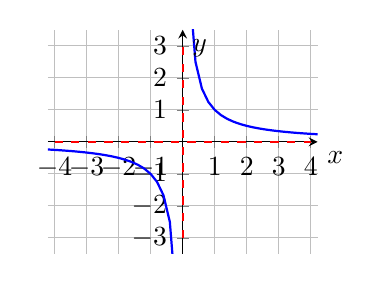
\begin{tikzpicture}
\begin{axis}[
    scale=0.5,
    xmin=-2.5, xmax=2.5,
    ymin=-3.5, ymax=3.5,
    axis lines=middle,
    axis equal,
    grid=both,
    xtick distance=1,
    ytick distance=1,
    xlabel=$x$,
    ylabel=$y$,
    xlabel style={at={(ticklabel* cs:1)}, anchor=north west},
    ylabel style={at={(ticklabel* cs:1)}, anchor=north west}
  ]
%  \addplot[blue,mark=none,thick=8pt] {x};
  \addplot[blue,mark=none,thick=8pt, domain=-5:-0.2] {1/x};
  \addplot[blue,mark=none,thick=8pt, domain=0.2:5] {1/x};
  \draw[red,dashed,thick=12pt] (axis cs:-4,0) -- (axis cs:4,0);
  \draw[red,dashed,thick=12pt] (axis cs:0,-3) -- (axis cs:0,3);
\end{axis}
\end{tikzpicture}
\end{center}

Свойства графика функции $y=\frac{1}{x}$:
\begin{enumerate}[nosep]
  \item График функции лежит в I и III координатных четвертях.
  \item График функции чертится движением карандаша/ручки слева направо сверху вниз.
  \item Оси координат являются асимптотами.
  \item Движение карандаша/ручки происходят с отрывом от бумаги при переходе через ось ординат. 
\end{enumerate}

\begin{exercises}
  \begin{question}
    Построить график функции:
    \begin{multicols}{2}
      \begin{enumerate}[label=\arabic*)]
      \item $y=\frac{2}{x}$
      \item $y=\frac{4}{x}$
      \item $y=\frac{10}{x}$
      \item $y=\frac{-2}{x}$
      \item $y=-\frac{4}{x}$
      \item $y=-\frac{-10}{-x}$
    \end{enumerate}
  \end{multicols}
\end{question}
\begin{question}
  Принадлежат ли графику каждой из построенных функций точки:\\
  A(-6; -8), B(12; -4), C(0,3; -16), D (0,4; -120). 
\end{question}
\begin{question}
  Найти абсциссу точки графика построенных функций с ординатой: 12; -6; 100.
\end{question}
\begin{question}
  Найти ординату точки графика построенных функций с абсциссой: -3; 6; 0,2.
\end{question}
\end{exercises}

\subsubsection*{Замечания по выполненным построениям}
\begin{center}
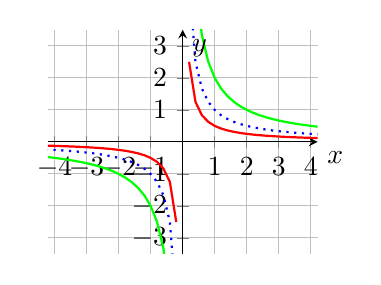
\begin{tikzpicture}
\begin{axis}[
    scale=0.5,
    xmin=-1.5, xmax=1.5,
    ymin=-3.5, ymax=3.5,
    axis lines=middle,
    axis equal,
    grid=both,
    xtick distance=1,
    ytick distance=1,
    xlabel=$x$,
    ylabel=$y$,
    xlabel style={at={(ticklabel* cs:1)}, anchor=north west},
    ylabel style={at={(ticklabel* cs:1)}, anchor=north west}
  ]
  \addplot[blue,mark=none,dotted,thick=8pt,domain=-5:-0.2] {1/x};
  \addplot[blue,mark=none,dotted,thick=8pt,domain=0.2:5] {1/x};
  \addplot[red,mark=none,thick=8pt,domain=-5:-0.2] {1/(2*x)};
  \addplot[red,mark=none,thick=8pt,domain=0.2:5] {1/(2*x)};
  \addplot[green,mark=none,thick=8pt,domain=-5:-0.2] {2/x};
  \addplot[green,mark=none,thick=8pt,domain=0.2:5] {2/x};
\end{axis}
\end{tikzpicture}
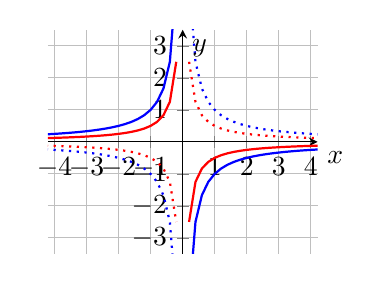
\begin{tikzpicture}
\begin{axis}[
    scale=0.5,
    xmin=-1.5, xmax=1.5,
    ymin=-3.5, ymax=3.5,
    axis lines=middle,
    axis equal,
    grid=both,
    xtick distance=1,
    ytick distance=1,
    xlabel=$x$,
    ylabel=$y$,
    xlabel style={at={(ticklabel* cs:1)}, anchor=north west},
    ylabel style={at={(ticklabel* cs:1)}, anchor=north west}
  ]
  \addplot[blue,mark=none,dotted,thick=8pt,domain=-5:-0.2] {1/x};
  \addplot[blue,mark=none,dotted,thick=8pt,domain=0.2:5] {1/x};
  \addplot[blue,mark=none,thick=8pt,domain=-5:-0.2] {-1/x};
  \addplot[blue,mark=none,thick=8pt,domain=0.2:5] {-1/x};
  \addplot[red,mark=none,dotted,thick=8pt,domain=-5:-0.2] {1/(2*x)};
  \addplot[red,mark=none,dotted,thick=8pt,domain=0.2:5] {1/(2*x)};
  \addplot[red,mark=none,thick=8pt,domain=-5:-0.2] {-1/(2*x)};
  \addplot[red,mark=none,thick=8pt,domain=0.2:5] {-1/(2*x)};
\end{axis}
\end{tikzpicture}
\end{center}

\begin{itemize}[nosep,leftmargin=0.5\labelwidth]
  \item Функция, график которой обладает свойством 2 гиперболы, называется \emph{убывающей}.
  \item Коэффициент пропорциональности k сужает график функции, если он больше 1 и растягивает, если меньше 1.
  \item Если коэффициент пропорциональности отрицательный, то график функции является зеркальным отражением графика функции относительно оси ординат или оси абсцисс.
\end{itemize}

%{\bf\color{blue}У П Р А Ж Н Е Н И Я}
%
%\begin{question}
%  Построить график функции:
%  \begin{multicols}{3}
%    \begin{enumerate}[label=\arabic*)]
%      \item $y=\frac{2}{x}$
%      \item $y=\frac{4}{x}$
%      \item $y=\frac{10}{x}$
%      \item $y=\frac{-2}{x}$
%      \item $y=-\frac{4}{x}$
%      \item $y=-\frac{-10}{-x}$
%    \end{enumerate}
%  \end{multicols}
%\end{question}
%\begin{question}
%  Принадлежат ли графику каждой из построенных функций точки: A(-6; -8), B(12; -4), C(0,3; -16), D (0,4; -120). 
%\end{question}
%
%\pagebreak
%\subsubsection*{Линейная и обратная линейная функция}
%
%Графиком линейной функции $y=kx+b$ является прямая линия, лежащая под углом $\alpha$ к оси абсцисс, где $\tg\alpha=k$, и пересекающая ось абсцисс в точке $\left(-\frac{k}{b},0\right)$. 
%
%\begin{enumerate}
%  \item Построить график функции
%  \begin{multicols}{3}
%    \begin{enumerate}[(1)]
%      \item $y=2x+1$
%      \item $y=4x+2$
%      \item $y=\frac{1}{2}x-1$
%      \item $y=-2x+1$
%      \item $y=-4x+2$
%      \item $y=-\frac{1}{2}x-1$
%    \end{enumerate}
%  \end{multicols}
%  \item Принадлежат ли графику каждой из построенных функций точки: A(-6; -8), B(12; -4), C(0,3; -16), D (0,4; -120). 
%  \item Найти абсциссу точки графика построенных функций с ординатой: 12; -6; 100.
%  \item Найти ординату точки графика построенных функций с абсциссой: -3; 6; 0,2.
%\end{enumerate}
%
%\hrule
%\medskip
%
%Графиком функции $y=\frac{1}{kx+b}$ является гипербола с вертикальной асимптотой, проходящей через точку $(-\frac{k}{b},0)$. 
%
%\begin{enumerate}
%  \item Построить график функции
%    \begin{multicols}{3}
%      \begin{enumerate}[(1)]
%        \item $y=\frac{1}{2x+1}$
%        \item $y=\frac{1}{2x+2}$
%        \item $y=\frac{1}{0.5x-2}$
%        \item $y=-\frac{1}{2x+1}$
%        \item $y=-\frac{1}{2x+2}$
%        \item $y=-\frac{1}{0.5x-2}$
%      \end{enumerate}
%    \end{multicols}
%  \item Принадлежат ли графику каждой из построенных функций точки: A(-6; -8), B(12; -4), C(0,3; -16), D (0,4; -120). 
%  \item Найти абсциссу точки графика построенных функций с ординатой: 12; -6; 100.
%  \item Найти ординату точки графика построенных функций с абсциссой: -3; 6; 0,2.
%\end{enumerate}
%
%\hrule
%\medskip
%
%\subsubsection*{Замечания по выполненным построениям}
%
%\begin{itemize}
%  \item Коэффициент пропорциональности k сужает график функции, если он больше 1 и растягивает, если больше 1.
%  \item Если коэффициент пропорциональности k отрицательный, то график функции является зеркальным отражением графика функции относительно оси ординат.
%  \item Добавление совободного члена приводит к смещению графика функции вправо или влево.
%\end{itemize}
\end{document}
